\begin{center}
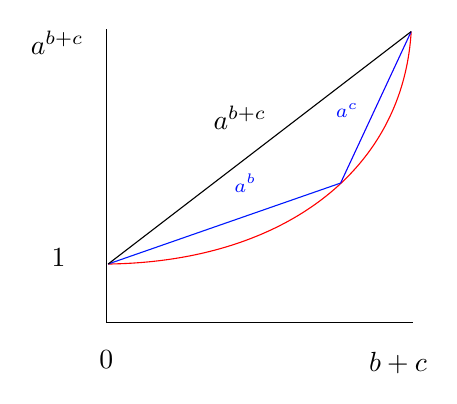
\begin{tikzpicture}[x=0.75pt,y=0.75pt,yscale=-1,xscale=1]
%uncomment if require: \path (0,300); %set diagram left start at 0, and has height of 300

%Curve Lines [id:da7648292128629934] 
\draw [color={rgb, 255:red, 255; green, 0; blue, 0 }  ,draw opacity=1 ]   (114.5,175) .. controls (197.5,174) and (256.5,131) .. (260.5,63) ;
%Straight Lines [id:da7623123576251518] 
\draw    (113.5,203) -- (261.5,203) ;
%Straight Lines [id:da45171993306474634] 
\draw    (113.5,62) -- (113.5,203) ;
%Straight Lines [id:da11496418575904588] 
\draw [color={rgb, 255:red, 0; green, 24; blue, 253 }  ,draw opacity=1 ]   (114.5,175) -- (226.5,136) ;
%Straight Lines [id:da9303796173825488] 
\draw [color={rgb, 255:red, 12; green, 0; blue, 255 }  ,draw opacity=1 ]   (260.5,63) -- (226.5,136) ;
%Straight Lines [id:da30716669420649056] 
\draw    (114.5,175) -- (260.5,63) ;

% Text Node
\draw (109,215.4) node [anchor=north west][inner sep=0.75pt]    {$0$};
% Text Node
\draw (239,216.4) node [anchor=north west][inner sep=0.75pt]    {$b+c$};
% Text Node
\draw (86,166.4) node [anchor=north west][inner sep=0.75pt]    {$1$};
% Text Node
\draw (164,97.4) node [anchor=north west][inner sep=0.75pt]    {$a^{b+c}$};
% Text Node
\draw (174,130.4) node [anchor=north west][inner sep=0.75pt]  [font=\scriptsize,color={rgb, 255:red, 0; green, 15; blue, 255 }  ,opacity=1 ]  {$a^{b}$};
% Text Node
\draw (223,96.4) node [anchor=north west][inner sep=0.75pt]  [font=\scriptsize,color={rgb, 255:red, 0; green, 15; blue, 255 }  ,opacity=1 ]  {$a^{c}$};
% Text Node
\draw (76,61.4) node [anchor=north west][inner sep=0.75pt]    {$a^{b+c}$};


\end{tikzpicture}
\end{center}